% !TeX program = xelatex
% !TeX encoding = UTF-8
% !TeX TXS-program:compile = txs:///xelatex | txs:///xelatex
\documentclass[aspectratio=169, table, 12pt]{beamer}

% Preamble bersama seluruh slide mata kuliah ini.
% Dipanggil dari slides/sessionXX/sessionXX.tex tepat sesudah baris
% \documentclass[aspectratio=169, table, 12pt]{beamer}
% Paket tambahan yang hanya dibutuhkan satu sesi ditulis di berkas sesi itu.

\usepackage{colortbl}
\usepackage{xcolor}
\usepackage{listings}
\usepackage{tabularx}
\usepackage{booktabs}
\usepackage{tikz}
\usepackage{pgfplots}
\usepackage{fontspec}
\usepackage[english,bahasai]{babel}
\pgfplotsset{compat=1.18}
\usetikzlibrary{arrows.meta, positioning, calc, fit, shapes.geometric,
  shapes.multipart, backgrounds, matrix, chains, trees}

\makeatletter
\def\input@path{{../theme/}}
\makeatother
\graphicspath{{../theme/}{../../figures/}}
% Stub symlink Windows memakai tema cadangan sampai aset institusi tersedia.
\IfFileExists{../theme/beamerthemePradita.sty}{%
  \usetheme{Pradita}
}{%
  \usetheme{Madrid}
  \setmainfont{TeX Gyre Heros}
  \setsansfont{TeX Gyre Heros}
  \setbeamertemplate{navigation symbols}{}
}

\definecolor{praditagreen}{RGB}{37, 113, 71}
\setbeamercolor{structure}{fg=praditagreen}
\setbeamercolor{palette primary}{bg=praditagreen,fg=white}
\setbeamercolor{palette secondary}{bg=praditagreen!80!black,fg=white}
\setbeamercolor{palette tertiary}{bg=praditagreen!60!black,fg=white}
\setbeamerfont{frametitle}{size=\large}
\setbeamertemplate{caption}[numbered]

% Ukuran header mengikuti teks agar judul panjang tidak menabrak logo.
\setbeamercolor{frametitle}{bg=white,fg=black}
\setbeamertemplate{frametitle}{%
  \begin{beamercolorbox}[wd=\paperwidth,sep=0.2cm]{frametitle}
    \begin{minipage}[c]{0.77\paperwidth}
      \raggedright\fontsize{16}{18}\selectfont\bfseries\insertframetitle
      \ifx\insertframesubtitle\empty\else
        \par\small\mdseries\insertframesubtitle
      \fi
    \end{minipage}\hfill
    \begin{minipage}[c]{0.15\paperwidth}
      \IfFileExists{../theme/classFiles/logo_universitas.png}{%
        
\includegraphics[width=\linewidth]{../theme/classFiles/logo_universitas.png}%
      }{}
    \end{minipage}
  \end{beamercolorbox}
}
\setbeamertemplate{footline}{%
  \ifnum\value{framenumber}>1
    \begin{beamercolorbox}[wd=\paperwidth,ht=0.35cm,dp=0.15cm,
      leftskip=0.3cm,rightskip=0.3cm]{palette primary}
      \footnotesize\bfseries\insertframenumber/\inserttotalframenumber
      \hfill IT40513
    \end{beamercolorbox}
  \fi
}
\DeclareRobustCommand{\berkas}[1]{\path{#1}}

% Tema membuat garis tabel berwarna putih. Dikembalikan agar tabel terbaca.
\arrayrulecolor{black}
\setlength{\arrayrulewidth}{0.5pt}

\lstdefinelanguage{yaml}{
  basicstyle=\ttfamily\scriptsize,
  keywordstyle=\color{blue}\bfseries,
  commentstyle=\color{gray}\itshape,
  stringstyle=\color{red},
  showstringspaces=false,
  breaklines=true,
  frame=lines,
  numbers=none,
  backgroundcolor=\color{lightgray!10},
  tabsize=2,
  morecomment=[l]{\#}
}

\lstdefinelanguage{json}{
  basicstyle=\ttfamily\scriptsize,
  stringstyle=\color{red},
  commentstyle=\color{gray},
  breaklines=true,
  showstringspaces=false,
  tabsize=2,
  numbers=none,
  frame=lines,
  backgroundcolor=\color{lightgray!10},
  string=[s]{"}{"}
}

\lstdefinelanguage{bash}{
  keywords={},
  basicstyle=\ttfamily\scriptsize,
  ndkeywords={docker, kubectl, helm, curl, git, terraform},
  ndkeywordstyle=\color{purple}\bfseries,
  sensitive=true,
  commentstyle=\color{gray},
  numbers=none,
  breaklines=true,
  frame=lines,
  backgroundcolor=\color{lightgray!10},
  tabsize=2,
  comment=[l]{\#},
  showstringspaces=false
}

\lstdefinelanguage{http}{
  keywords={GET, POST, PUT, PATCH, DELETE, HEAD, OPTIONS, HTTP},
  basicstyle=\ttfamily\scriptsize,
  keywordstyle=\color{blue}\bfseries,
  sensitive=true,
  numbers=none,
  breaklines=true,
  frame=lines,
  backgroundcolor=\color{lightgray!10},
  tabsize=2,
  showstringspaces=false
}

\subtitle{IT40513 · Enterprise Architecture \& Digital Blueprint}
\author{\textbf{Alfa Yohannis}}


% Sampul membatasi judul di panel putih tema rujukan Pradita.
\setbeamertemplate{title page}{%
  \begin{tikzpicture}[remember picture,overlay]
    \node[anchor=north west,inner sep=0pt,text width=8.8cm]
      at ([xshift=1cm,yshift=-3.15cm]current page.north west) {%
        {\small\insertsubtitle\par}\vspace{0.25cm}
        \resizebox{8.8cm}{!}{\begin{minipage}{12cm}
          \raggedright\color{praditagreen}\bfseries\inserttitle
        \end{minipage}}
      };
    \node[anchor=south west,inner sep=0pt]
      at ([xshift=1cm,yshift=1.65cm]current page.south west)
      {\small\insertdate};
    \node[anchor=west,inner sep=0pt,text=white]
      at ([xshift=0.8cm,yshift=0.75cm]current page.south west)
      {\small\insertauthor};
  \end{tikzpicture}
}


% Batasi kedua dimensi gambar agar diagram bersama tetap berada pada slide.
\newsavebox{\eafigbox}
\newcommand{\eadiagram}[1]{%
  \sbox{\eafigbox}{\resizebox{0.94\textwidth}{!}{\input{#1}}}%
  \ifdim\dimexpr\ht\eafigbox+\dp\eafigbox\relax>0.64\textheight
    \resizebox{!}{0.64\textheight}{\usebox{\eafigbox}}%
  \else
    \usebox{\eafigbox}%
  \fi
}


\title{\Huge Arsitektur Data dan\\ \vspace{10pt} Informasi Saat Ini}
\date{Pertemuan 06}

\begin{document}

\frame{\titlepage}

\begin{frame}
  \frametitle{Isi Pertemuan}
  \vspace{14pt}
  \begin{columns}[t]
    \column{0.5\textwidth}
    {\small\tableofcontents[sections={1-3}]}

    \column{0.5\textwidth}
    {\small\tableofcontents[sections={4-6}]}
  \end{columns}
\end{frame}

\begin{frame}{\hfill}
  \centering
  \Huge{\textbf{Satu bulan, dua angka:\\kunjungan mana\\yang benar?}}
\end{frame}

\section{Tujuan dan Konteks}

\begin{frame}{\hfill}
  \centering
  \Huge{\textbf{Tujuan dan Konteks}}
\end{frame}

\begin{frame}{{\Large Tujuan Pembelajaran}}
  \vspace{10pt}
  \begin{itemize}
    \item Mengidentifikasi konsep informasi bisnis utama beserta pemiliknya.
    \item Memetakan lokasi dan aliran data penting di antara aplikasi dengan matriks CRUD
          (\textit{Create, Read, Update, Delete}).
    \item Menganalisis masalah kualitas, duplikasi, dan klasifikasi data yang menghambat strategi.
  \end{itemize}
\end{frame}

\begin{frame}{{\Large Rapat yang Berhenti di Satu Angka}}
  \vspace{6pt}
  \small
  \begin{itemize}
    \item November 2025: Direktur Keuangan melaporkan 99.870 kunjungan Oktober, Direktur Pelayanan
          membawa 102.640.
    \item Selisihnya 2.770 kunjungan, dan tidak ada yang salah menghitung. Arti ``kunjungan'' berbeda.
    \item Akar masalahnya: data pasien tersebar di lima SIMRS (Sistem Informasi Manajemen Rumah Sakit),
          Medikara+, ERP keuangan, dan puluhan berkas \textit{spreadsheet}.
    \item Pekerjaan ini termasuk fase C pada ADM (\textit{Architecture Development Method}) untuk
          \textit{baseline}.
    \item Hasilnya untuk C2: peta informasi, matriks CRUD, dan daftar masalah data.
  \end{itemize}
\end{frame}

\begin{frame}{{\Large Diagram Konsep Bab 6}}
  \centering
  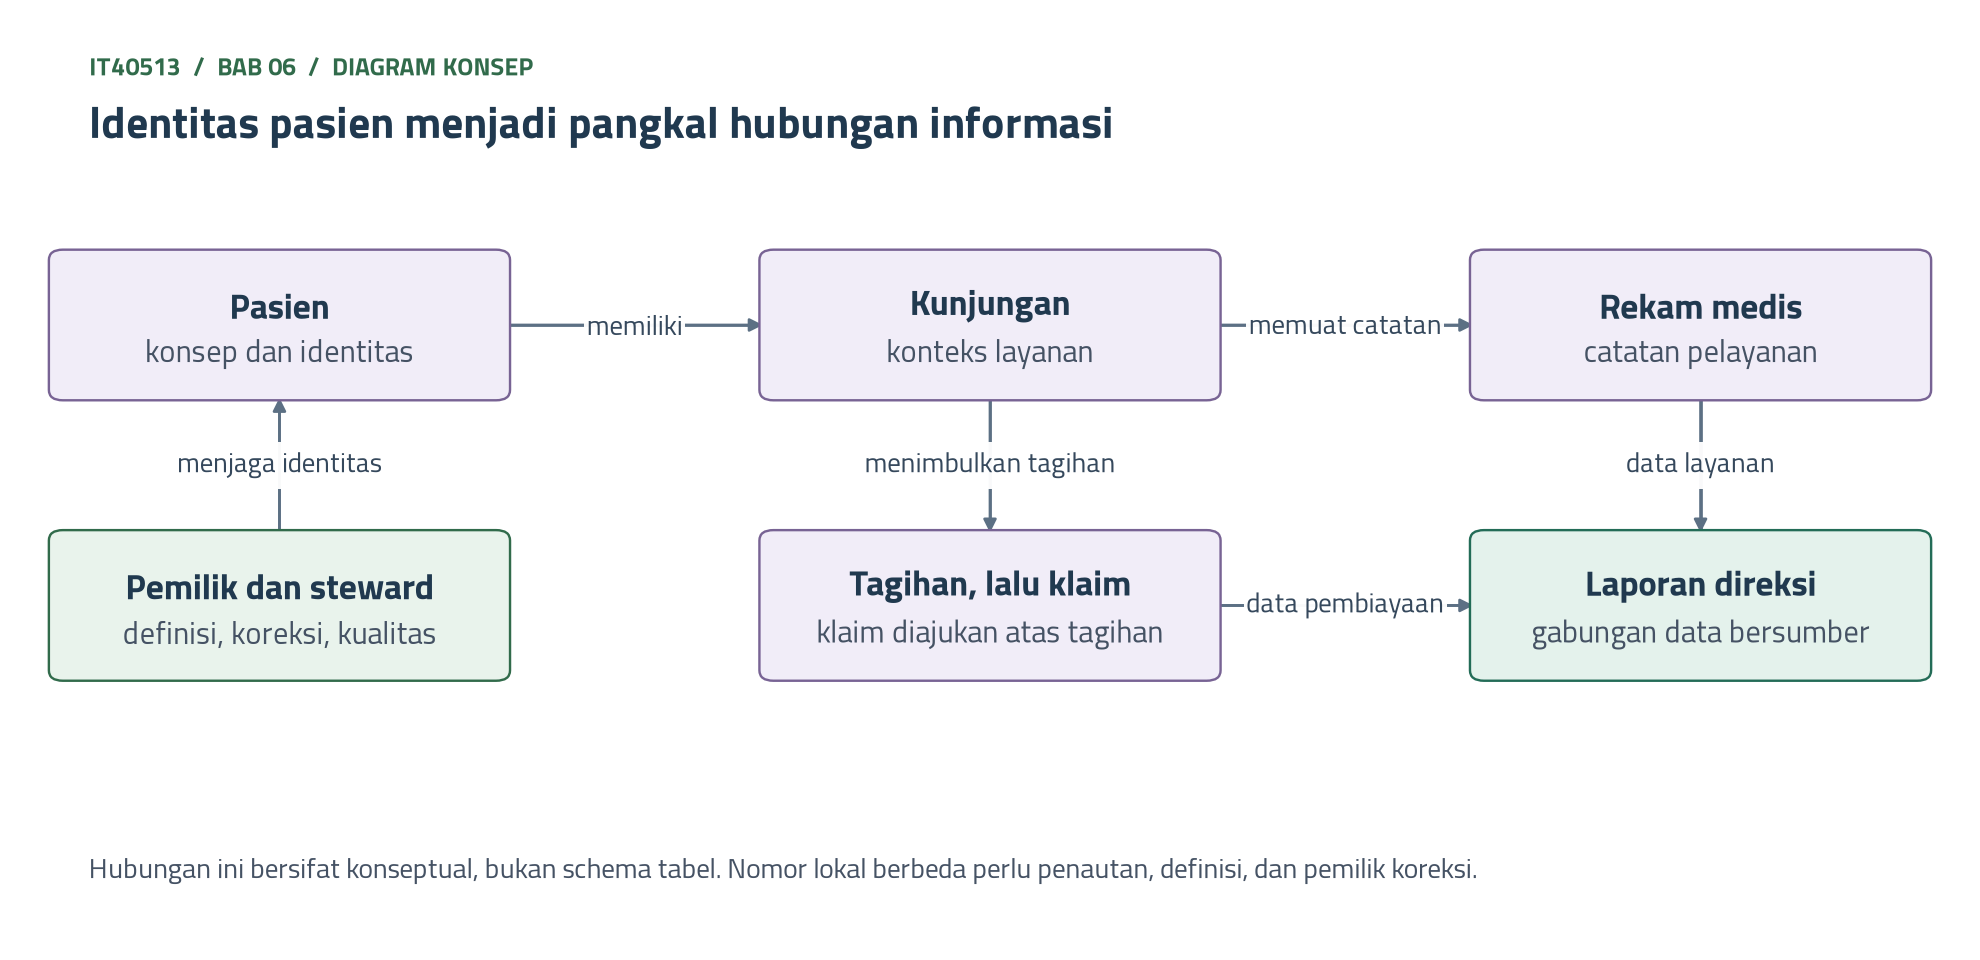
\includegraphics[width=0.96\textwidth,height=0.77\textheight,keepaspectratio]{../../figures/ch06-diagram-konsep.png}
  \label{fig:session06-ilustrasi-bab}
\end{frame}

\section{Konsep Informasi Bisnis}

\begin{frame}{\hfill}
  \centering
  \Huge{\textbf{Konsep Informasi Bisnis}}
\end{frame}

\begin{frame}{{\Large Data, Informasi, dan Konsep Bisnis}}
  \footnotesize
  \begin{tabularx}{\textwidth}{lXX}
    \hline
    \textbf{Istilah} & \textbf{Pengertian} & \textbf{Contoh di Medikara} \\
    \hline
    Data & Nilai yang tercatat, belum bermakna tanpa konteks & Angka 38,5; teks
      JKT-0045821 \\
    \hline
    Informasi & Data yang diberi konteks sehingga dapat dipakai untuk memutuskan &
      Suhu pasien anak naik dari 37,2 menjadi 38,5 derajat dalam 10 jam \\
    \hline
    Konsep bisnis & Hal yang dibicarakan organisasi dengan arti yang disepakati &
      Pasien, Kunjungan, Rekam Medis, Klaim \\
    \hline
  \end{tabularx}

  \vspace{8pt}
  \small Arsitektur data bekerja pada tingkat konsep bisnis.
\end{frame}

\begin{frame}{{\Large Peta Informasi dan Arti yang Disepakati}}
  \vspace{6pt}
  \small
  \begin{itemize}
    \item Konsep informasi: hal yang perlu diketahui organisasi untuk menjalankan kapabilitasnya.
    \item Peta informasi: kumpulan konsep beserta hubungan, tipe, dan keadaannya.
    \item Analogi: bagian definisi pada kontrak sewa rumah, disepakati sebelum pasal dibaca.
    \item Kunjungan: SIMRS Jakarta mencatat per poliklinik, SIMRS Bandung per pasien per hari. Selisih
          2.770 berasal dari 1.980 telekonsultasi dan 790 kunjungan ke lebih dari satu poliklinik.
    \item Pasien: satu akun Medikara+ dapat mendaftarkan sampai lima anggota keluarga.
  \end{itemize}
\end{frame}

\begin{frame}{{\Large Model Data Konseptual Inti Medikara}}
  \centering
  \eadiagram{../../figures/ch06-model-konseptual.tex}

  \vspace{4pt}
  {\small Dibaca dari tengah. Kesalahan identitas pasien merambat ke seluruh rantai.\par}
\end{frame}

\begin{frame}{{\Large Satu Konsep, Enam Tempat}}
  \centering
  {\small \textit{Business object} mewakili konsep bisnis, \textit{data object} mewakili data di satu
  aplikasi, dan \textit{artifact} mewakili wujud fisiknya.\par}
  \vspace{4pt}
  \eadiagram{../../figures/ch06-objek-archimate.tex}
\end{frame}

\begin{frame}{{\Large Kasus: Enam Konsep Inti}}
  \begin{block}{Kasus Medikara Health}
    \footnotesize
    \begin{enumerate}
      \item Pasien: orang yang terdaftar untuk menerima layanan kesehatan di fasilitas Medikara.
      \item Kunjungan: satu peristiwa pelayanan pada satu fasilitas pada satu hari, termasuk
            telekonsultasi.
      \item Rekam Medis: kumpulan catatan klinis seorang pasien dari seluruh kunjungannya.
      \item Resep: perintah dokter untuk pemberian obat dalam satu kunjungan.
      \item Tagihan: rincian biaya satu kunjungan yang dibayar pasien atau penjaminnya.
      \item Klaim: permintaan pembayaran atas tagihan kepada penjamin.
    \end{enumerate}
    Dengan Dokter, Fasilitas, dan Penjamin, peta informasi berisi sembilan konsep.
  \end{block}
\end{frame}

\section{Data Induk dan Kepemilikan}

\begin{frame}{\hfill}
  \centering
  \Huge{\textbf{Data Induk dan\\Kepemilikan}}
\end{frame}

\begin{frame}{{\Large Data Induk, Referensi, dan Transaksi}}
  \scriptsize
  \begin{tabularx}{\textwidth}{lXXX}
    \hline
    \textbf{Jenis} & \textbf{Ciri} & \textbf{Contoh} & \textbf{Akibat bila salah} \\
    \hline
    Data induk & Entitas inti, dipakai banyak proses, jarang berubah &
      Pasien, Dokter, Fasilitas & Menyebar ke semua transaksi yang merujuknya \\
    \hline
    Data referensi & Daftar nilai baku untuk mengelompokkan data lain &
      Jenis penjamin, kode poliklinik, kode wilayah &
      Laporan tidak dapat dijumlahkan lintas rumah sakit \\
    \hline
    Data transaksi & Catatan kejadian, jumlahnya terus bertambah &
      Kunjungan, Resep, Tagihan, Klaim & Terbatas pada kejadian itu \\
    \hline
  \end{tabularx}

  \vspace{8pt}
  \small Sekitar 1,2 juta kunjungan per tahun kali rata-rata empat catatan: sekitar 4,8 juta catatan per
  tahun bergantung pada identitas pasien.

  \vspace{6pt}
  Analogi: buku induk siswa, daftar kode mata pelajaran, dan lembar presensi harian.
\end{frame}

\begin{frame}{{\Large Pemilik, Steward, dan Pengelola Teknis}}
  \scriptsize
  \begin{tabularx}{\textwidth}{lXX}
    \hline
    \textbf{Peran} & \textbf{Tanggung jawab} & \textbf{Untuk konsep Pasien} \\
    \hline
    Pemilik bisnis & Memutuskan definisi, mutu minimum, dan hak akses &
      Saat ini direktur tiap rumah sakit, sehingga ada lima pemilik \\
    \hline
    \textit{Data steward} & Menjaga mutu sehari-hari, memperbaiki data, memeriksa
      calon duplikat & Kepala pendaftaran tiap rumah sakit \\
    \hline
    Pengelola teknis & Menyimpan, mencadangkan, dan memasang hak akses sesuai
      keputusan pemilik & Tim TI tiap rumah sakit, vendor SIMRS, dan vendor
      Medikara+ \\
    \hline
  \end{tabularx}

  \vspace{8pt}
  \small Bagian TI biasanya pengelola, bukan pemilik. Bila dianggap pemilik, keputusan akses diambil oleh
  orang yang tidak memikul akibat klinis maupun hukumnya.
\end{frame}

\begin{frame}{{\Large Stewardship dan Hak Memutuskan}}
  \vspace{6pt}
  \small
  \begin{itemize}
    \item Khatri dan Brown: tata kelola data adalah soal hak memutuskan, dalam lima ranah: prinsip data,
          kualitas data, metadata, akses data, dan siklus hidup data.
    \item Saat memotret kondisi saat ini: siapa yang memutuskan, walaupun jawabannya ``tidak ada''.
    \item \textit{Stewardship} berbeda dari proyek pembersihan data yang dijalankan sekali.
    \item Kepala pendaftaran RS Bekasi: rata-rata 60 calon duplikat per minggu, sekitar 25 terbukti orang
          yang sama.
    \item \textit{Steward} data referensi memperbarui kode jenis penjamin sekali untuk lima rumah sakit.
  \end{itemize}
\end{frame}

\begin{frame}{{\Large Satu Orang, Tiga Nomor}}
  \centering
  \eadiagram{../../figures/ch06-identitas-ganda.tex}
\end{frame}

\begin{frame}{{\Large Kasus: Lima Pola Nomor Rekam Medis}}
  \begin{block}{Kasus Medikara Health}
    \small
    \begin{itemize}
      \item Tiap rumah sakit membawa pola sendiri, misalnya \texttt{JKT-0045821} dan \texttt{BKS-118204}.
      \item NIK (Nomor Induk Kependudukan) tidak wajib diisi pada pendaftaran sebelum 2020.
      \item Misalkan sampel acak 10.000 nomor aktif: 1.140 nomor, atau 11,4 persen, milik orang yang sudah
            punya nomor di rumah sakit lain.
      \item Dokter tidak melihat riwayat dari rumah sakit lain. Laporan menghitung orang yang sama lebih
            dari sekali.
      \item Pemilik konsep Pasien ada lima orang, sehingga tidak ada yang berwenang menetapkan satu aturan
            penomoran.
    \end{itemize}
  \end{block}
\end{frame}

\section{Lokasi dan Aliran Data}

\begin{frame}{\hfill}
  \centering
  \Huge{\textbf{Lokasi dan Aliran Data}}
\end{frame}

\begin{frame}{{\Large Aliran yang Tidak Tercatat}}
  \vspace{6pt}
  \small
  \begin{itemize}
    \item Dua staf perencanaan mengunduh tujuh ekspor: tiap SIMRS, ERP, dan Medikara+.
    \item Ekspor diambil setelah tutup buku hari kerja kelima, digabung enam hari kerja, lalu laporan
          terbit pada hari kerja ke-12.
    \item Biayanya 12 hari-orang per bulan, atau 144 hari-orang per tahun.
    \item TOGAF menyediakan \textit{Data Dissemination diagram} dan \textit{Application/Data matrix}. Yang
          digambar adalah aliran yang sungguh terjadi.
    \item Analogi: selang yang dipasang warga sendiri tidak ada di peta saluran air resmi.
  \end{itemize}
\end{frame}

\begin{frame}{{\Large Aliran Data Tingkat Tinggi Medikara}}
  \centering
  \eadiagram{../../figures/ch06-aliran-data.tex}
\end{frame}

\begin{frame}{{\Large Matriks CRUD Medikara Saat Ini}}
  \footnotesize
  \begin{tabularx}{\textwidth}{Xcccc}
    \hline
    \textbf{Konsep} & \textbf{SIMRS (5)} & \textbf{Medikara+} & \textbf{ERP} &
      \textbf{\textit{Spreadsheet}} \\
    \hline
    Pasien & CRU & CRU & R & R \\
    \hline
    Janji Temu & RU & CRUD & & \\
    \hline
    Kunjungan & CRU & CR & & R \\
    \hline
    Rekam Medis & CRU & CR & & \\
    \hline
    Hasil Laboratorium & CRU & R & & R \\
    \hline
    Resep & CRU & R & & \\
    \hline
    Jadwal Praktik Dokter & CRUD & R & & \\
    \hline
    Tagihan & CRU & R & RU & R \\
    \hline
    Klaim & CRU & & R & CRU \\
    \hline
    Kontrak Penjamin & R & & R & CRUD \\
    \hline
  \end{tabularx}

  \vspace{6pt}
  \small C membuat, R membaca, U mengubah, D menghapus. Kolom SIMRS mewakili lima aplikasi.
\end{frame}

\begin{frame}{{\Large Lima Pola pada Matriks CRUD}}
  \footnotesize
  \begin{tabularx}{\textwidth}{XXX}
    \hline
    \textbf{Pola} & \textbf{Artinya} & \textbf{Contoh di Medikara} \\
    \hline
    C di lebih dari satu kolom & Ada beberapa versi kebenaran yang harus
      disatukan belakangan & Pasien, Kunjungan, Rekam Medis, Klaim \\
    \hline
    C hanya di kolom \textit{spreadsheet} & Data penting di luar aplikasi yang
      dikelola, biasanya tanpa pemilik & Kontrak Penjamin \\
    \hline
    R di kolom \textit{spreadsheet} & Aliran manual yang tidak tercatat di
      diagram integrasi & Pasien, Kunjungan, Hasil Laboratorium, Tagihan \\
    \hline
    Tidak ada D di baris mana pun & Data tidak pernah dihapus, wajar bila
      diwajibkan aturan masa simpan & Rekam Medis, Resep, Tagihan \\
    \hline
    Tidak ada C sama sekali & Data datang dari luar atau masih dicatat di
      kertas & Tidak ditemukan pada contoh ini \\
    \hline
  \end{tabularx}
\end{frame}

\begin{frame}{{\Large Membaca Pola Matriks}}
  \vspace{6pt}
  \small
  \begin{itemize}
    \item Pasien, Kunjungan, dan Rekam Medis masing-masing dibuat di enam tempat: lima SIMRS dan Medikara+.
    \item Klaim BPJS Kesehatan dibuat di SIMRS, klaim asuransi swasta direkap di \textit{spreadsheet}.
    \item Kontrak Penjamin dengan BPJS Kesehatan dan 14 perusahaan asuransi hanya dibuat di satu
          \textit{spreadsheet} milik bagian keuangan.
    \item Huruf R di kolom \textit{spreadsheet} tidak aman: salinan data berpindah ke laptop staf, surel,
          dan folder bersama.
    \item \textit{Spreadsheet} harus muncul di peta agar biayanya terlihat.
  \end{itemize}
\end{frame}

\section{Klasifikasi dan Kualitas Data}

\begin{frame}{\hfill}
  \centering
  \Huge{\textbf{Klasifikasi dan\\Kualitas Data}}
\end{frame}

\begin{frame}{{\Large Skema Klasifikasi Empat Tingkat}}
  \scriptsize
  \begin{tabularx}{\textwidth}{lXXX}
    \hline
    \textbf{Tingkat} & \textbf{Arti} & \textbf{Contoh} & \textbf{Perlakuan minimum} \\
    \hline
    Publik & Boleh diketahui siapa pun & Daftar layanan, tarif umum, alamat
      fasilitas & Tanpa pembatasan baca, perubahan lewat pemilik \\
    \hline
    Internal & Untuk karyawan, kerugian kecil bila bocor & SOP (\textit{Standard
      Operating Procedure}), materi pelatihan & Hanya akun karyawan \\
    \hline
    Rahasia & Kerugian nyata bagi organisasi atau orang bila bocor & Identitas
      pasien, laporan pendapatan, kontrak penjamin & Akses menurut peran,
      tercatat, tidak di perangkat pribadi \\
    \hline
    Sangat Rahasia & Kerugian berat, termasuk data pribadi spesifik & Rekam
      medis, diagnosis, catatan telekonsultasi & Akses seperlunya, dienkripsi,
      tiap akses dicatat, berbagi hanya lewat perjanjian \\
    \hline
  \end{tabularx}

  \vspace{6pt}
  \small Analogi: lobi, ruang staf, ruang arsip rekam medis, dan lemari obat narkotika.
\end{frame}

\begin{frame}{{\Large Dua Sumbu: Tingkat dan Kategori}}
  \vspace{6pt}
  \small
  \begin{itemize}
    \item Tingkat klasifikasi adalah keputusan organisasi. Kategori data pribadi adalah ketentuan
          undang-undang.
    \item UU 27/2022 Pasal 4, data pribadi spesifik: kesehatan, biometrik, genetika, catatan kejahatan,
          data anak, keuangan pribadi, dan data lain sesuai peraturan.
    \item Data pribadi umum: nama lengkap, jenis kelamin, kewarganegaraan, agama, status perkawinan, dan
          data yang dikombinasikan.
    \item Rencana akuisisi klinik tergolong Rahasia, walaupun bukan data pribadi.
    \item Nama dokter adalah data pribadi umum, tetapi dapat tergolong Publik.
  \end{itemize}
\end{frame}

\begin{frame}{{\Large Ketentuan yang Membentuk Arsitektur Data}}
  \scriptsize
  \begin{tabularx}{\textwidth}{>{\raggedright\arraybackslash}p{2.7cm}XX}
    \hline
    \textbf{Ketentuan} & \textbf{Isi singkat} & \textbf{Akibat bagi arsitektur data} \\
    \hline
    UU 27/2022 Pasal 4 & Data kesehatan dan data keuangan pribadi termasuk data
      pribadi spesifik & Rekam Medis, Hasil Laboratorium, Resep, dan Klaim diberi
      label spesifik \\
    \hline
    Peraturan Menteri Kesehatan (Permenkes) 24/2022 Pasal 3 ayat (1) & Setiap fasilitas pelayanan kesehatan
      wajib menyelenggarakan rekam medis elektronik & Catatan klinis di kertas
      atau \textit{spreadsheet} tidak memenuhi \\
    \hline
    Pasal 21 & Rekam medis elektronik harus terhubung dengan platform
      interoperabilitas Kementerian Kesehatan & Kelima SIMRS wajib mampu
      mengirim data ke SATUSEHAT \\
    \hline
    Pasal 25 ayat (1) & Dokumen rekam medis milik fasilitas, sedangkan isinya
      milik pasien & Permintaan pasien harus dapat dijawab dari semua tempat
      penyimpanan \\
    \hline
    Pasal 39 ayat (1) & Rekam medis elektronik disimpan paling singkat 25 tahun
      sejak kunjungan terakhir & Data harus bertahan lebih lama daripada
      aplikasinya \\
    \hline
    Pasal 45 & Penyesuaian paling lambat 31 Desember 2023 & Kewajiban sudah
      berlaku penuh \\
    \hline
  \end{tabularx}

  \vspace{6pt}
  \small Bila kunjungan tetap 1,2 juta per tahun, dalam 25 tahun ada paling sedikit 30 juta catatan.
\end{frame}

\begin{frame}{{\Large Kasus: Kebocoran Lewat Vendor}}
  \begin{block}{Kasus Medikara Health}
    \small
    \begin{itemize}
      \item Data latihan IT40613 Bab 6: akun dukungan vendor, API bawaan SIMRS di dua rumah sakit,
            155 panggilan per malam selama 8 malam, 1.240 rekam kunjungan.
      \item Rekam Medis juga berada di basis data vendor, tetapi tidak tercatat di dokumen Medikara.
      \item Rekam kunjungan tergolong Sangat Rahasia, tetapi labelnya belum pernah dipasang.
      \item Tidak ada pemilik bisnis yang berwenang menilai akses setelah kontrak selesai.
      \item Aliran ke akun dukungan vendor tidak muncul di diagram aliran mana pun.
    \end{itemize}
  \end{block}
\end{frame}

\begin{frame}{{\Large Lima Dimensi Kualitas Data}}
  \scriptsize
  \begin{tabularx}{\textwidth}{lXXX}
    \hline
    \textbf{Dimensi} & \textbf{Pertanyaan} & \textbf{Ukuran di Medikara} & \textbf{Dampak} \\
    \hline
    Akurasi & Apakah nilainya sesuai kenyataan? & 4,2\% dari 2.000 alamat
      sampel tidak sesuai kartu identitas & Surat hasil pemeriksaan salah
      alamat \\
    \hline
    Kelengkapan & Apakah kolom wajib terisi? & NIK kosong pada 9\% pasien yang
      terdaftar sebelum 2020 & Tidak dapat memperoleh Nomor SATUSEHAT Pasien \\
    \hline
    Konsistensi & Apakah dua sumber sepakat? & Kunjungan Oktober 2025: 99.870
      di SIMRS, 102.640 di laporan & Direksi ragu memakai angka \\
    \hline
    Ketepatan waktu & Apakah data tersedia saat dibutuhkan? & Laporan terbit
      hari kerja ke-12; data ke SATUSEHAT rata-rata 3 hari & Keputusan bulan
      berjalan memakai angka bulan lalu \\
    \hline
    Keunikan & Apakah satu orang tercatat sekali? & 11,4\% dari 10.000 nomor
      rekam medis sampel adalah duplikat lintas rumah sakit & Riwayat klinis
      terpecah, jumlah pasien terlalu besar \\
    \hline
  \end{tabularx}

  \vspace{6pt}
  \small Angkanya adalah pengukuran awal yang diandaikan. Tiap tim mengukur ulang pada organisasinya.
\end{frame}

\begin{frame}{{\Large Identitas Ganda dan Dampaknya}}
  \vspace{6pt}
  \small
  \begin{itemize}
    \item Salah pisah: satu orang tercatat sebagai dua pasien atau lebih, sehingga riwayat terpecah.
    \item Salah gabung: dua orang tercatat sebagai satu pasien. Lebih jarang, tetapi lebih berbahaya.
    \item Layanan: misalkan 5 persen pasien rujukan antarrumah sakit menjalani pemeriksaan laboratorium
          ulang.
    \item Laporan: selisih 2,8 persen membuat setiap laporan diperiksa ulang.
    \item Klaim: misalkan 3,5 persen dari sekitar 40.000 berkas per bulan dikembalikan. Hasilnya 1.400
          berkas dan sekitar 350 jam kerja.
  \end{itemize}
\end{frame}

\begin{frame}{{\Large Daftar Masalah Data}}
  \scriptsize
  \begin{tabularx}{\textwidth}{lXlXX}
    \hline
    \textbf{No} & \textbf{Masalah} & \textbf{Dimensi} & \textbf{Bukti} & \textbf{Dampak pada strategi} \\
    \hline
    1 & Satu orang punya nomor di beberapa rumah sakit & Keunikan & 11,4\% dari
      sampel 10.000 & Menghambat ``Satu Pasien, Satu Rekam Medis'' \\
    \hline
    2 & Angka kunjungan SIMRS dan laporan berbeda & Konsistensi & Selisih 2.770
      pada Oktober 2025 & Direksi ragu memakai angka untuk investasi \\
    \hline
    3 & Kontrak penjamin hanya di \textit{spreadsheet} & Kepemilikan & C hanya
      di kolom \textit{spreadsheet} & Ekosistem mitra asuransi sulit
      diperluas \\
    \hline
  \end{tabularx}

  \vspace{8pt}
  \small Setiap masalah punya bukti berangka, atau diberi tanda ``perlu diukur''. Dampak ditulis terhadap
  strategi organisasi, bukan terhadap sistem.
\end{frame}

\section{Aktivitas dan Latihan}

\begin{frame}{\hfill}
  \centering
  \Huge{\textbf{Aktivitas dan Latihan}}
\end{frame}

\begin{frame}{{\Large Aktivitas: Menelusuri Data Pasien}}
  \vspace{6pt}
  \small
  \begin{itemize}
    \item Analis bisnis menentukan definisi dan pemilik bisnis. Analis teknologi menelusuri aplikasi,
          termasuk \textit{spreadsheet} dan aplikasi vendor.
    \item Pemodel memodelkan \textit{business object} dan \textit{data object} di Archi. Koordinator
          merangkum daftar masalah data.
    \item Susun 10 sampai 15 konsep, lalu tentukan pemilik, \textit{steward}, dan jenis datanya.
    \item Isi matriks CRUD, gambar aliran data, lalu beri tingkat klasifikasi dan kategori data pribadi.
    \item Ukur minimal dua dimensi kualitas dengan sampel yang dianonimkan.
  \end{itemize}
\end{frame}

\begin{frame}{{\Large Luaran C2 dan Kriteria Penilaian}}
  \footnotesize
  \begin{tabularx}{\textwidth}{Xr}
    \hline
    \textbf{Kriteria} & \textbf{Bobot} \\
    \hline
    Katalog konsep lengkap, definisinya jelas, dan setiap konsep punya pemilik
      atau catatan bahwa pemiliknya belum ada & 25\% \\
    \hline
    Matriks CRUD dan diagram aliran memuat aliran manual dan aplikasi vendor &
      25\% \\
    \hline
    Klasifikasi dan kategori data pribadi tepat, disertai alasan & 20\% \\
    \hline
    Daftar masalah data berbukti angka dan dikaitkan dengan strategi & 20\% \\
    \hline
    Nama konsep konsisten di seluruh artefak dan model Archi & 10\% \\
    \hline
  \end{tabularx}

  \vspace{6pt}
  \small Yang dicatat adalah konsep, jumlah, dan persentase, bukan isi data. Berkas pendukung:
  \berkas{sources/chapter06/README.md}.
\end{frame}

\begin{frame}{{\Large Ringkasan}}
  \vspace{6pt}
  \small
  \begin{itemize}
    \item Selisih 2.770 kunjungan berasal dari dua arti ``kunjungan'', bukan dari salah hitung.
    \item Identitas pasien adalah data induk paling penting, tetapi kini punya lima pemilik.
    \item Pasien dan Rekam Medis masing-masing dibuat di enam tempat. Laporan direksi bergantung pada
          aliran manual 144 hari-orang per tahun.
    \item Tingkat klasifikasi adalah keputusan organisasi. Kategori data pribadi ditetapkan UU 27/2022.
    \item Pesan utama: data yang tidak diketahui tempatnya, pemiliknya, dan sensitivitasnya tidak dapat
          dilindungi, tidak dapat dipercaya, dan tidak dapat dipindahkan ke kondisi target.
  \end{itemize}
\end{frame}

\begin{frame}{{\Large Latihan}}
  \vspace{6pt}
  \small
  \begin{enumerate}
    \item Dampak Nomor Rekam Medis Sendiri-Sendiri: rumah sakit Jakarta, Bekasi, dan Depok memberi nomor
          sendiri-sendiri. Tuliskan dampak pada layanan pasien, laporan manajemen, dan kepatuhan, beserta
          skalanya.
    \item Menemukan Data Tanpa Pemilik dengan Matriks CRUD: cari baris yang C-nya hanya di kolom
          \textit{spreadsheet}, C-nya di lebih dari satu kolom, atau pemiliknya kosong.
    \item Mengklasifikasikan Tiga Jenis Data: jadwal praktik dokter, hasil laboratorium, dan nomor
          rekening karyawan. Tentukan kategori dan tingkat klasifikasinya.
  \end{enumerate}
\end{frame}

\begin{frame}{{\Large Bacaan dan Berkas Pendukung}}
  \vspace{10pt}
  \begin{itemize}
    \item \href{https://www.opengroup.org/togaf}{\textit{The TOGAF Standard, 10th Edition (2025 Update)}}
    \item \href{https://cdn.ymaws.com/www.businessarchitectureguild.org/resource/resmgr/bizbok15/BIZBOKv15_introduction.pdf}{\textit{A Guide to the Business Architecture Body of Knowledge (BIZBOK Guide), Version 15}}
    \item \href{https://publications.opengroup.org/standards/archimate/c226}{\textit{ArchiMate 3.2 Specification}}
    \item \berkas{sources/chapter06/README.md}
  \end{itemize}
\end{frame}

\end{document}
